	
\part{Cinética de crescimento}
	\chapter{SAXS resolvido no tempo}
	
	As curvas médias de SAXS nas aquisições de 1-30 estão presentes nas figuras 
	\begin{figure}[h]
		\begin{subfigure}[t]{0.5\textwidth}
			\centering
			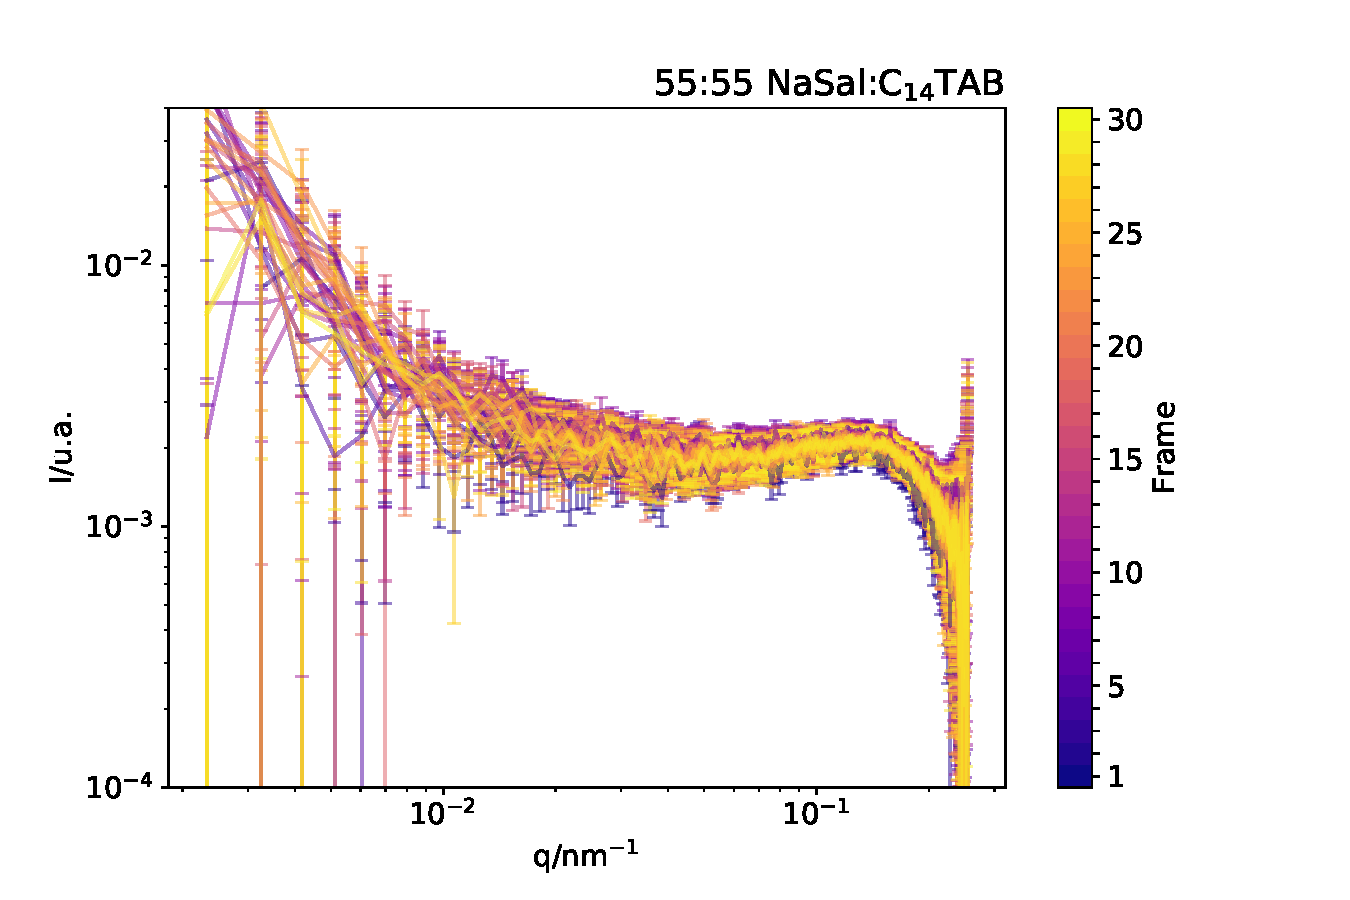
\includegraphics[width=\textwidth]{imagens/saxs/TR_saxs_55_55_dados.pdf}
			\caption{Dados}
			\label{fig:saxs_tr_55_d}
		\end{subfigure}%
		\begin{subfigure}[t]{0.5\textwidth}
			\centering
			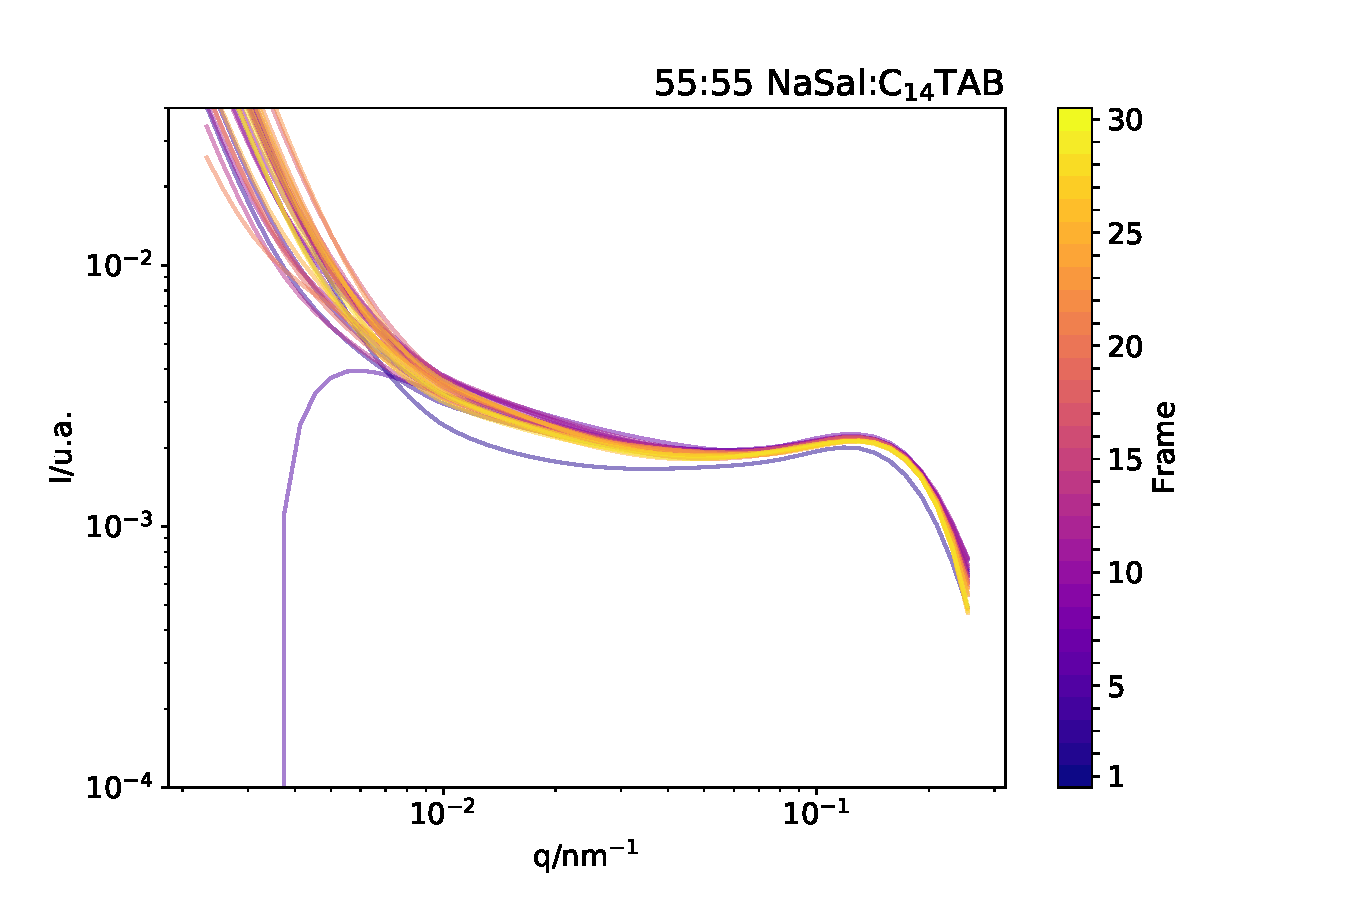
\includegraphics[width=\textwidth]{imagens/saxs/TR_saxs_55_55_ajuste.pdf}
			\caption{Ajustes}
			\label{fig:saxs_tr_55_a}
		\end{subfigure}
		\caption{Dados experimentais médios das curvas de SAXS nas aquisições numeradas de 1-30, numeradas do menor ao maior tempo de espera. As curvas foram obtidas pela mistura de 55 \mM{} de NaSal com 55\mM{} de TTAB.}
		\label{fig:saxs_tr_55}
	\end{figure} 

	\begin{figure}[h]
		\begin{subfigure}[t]{0.5\textwidth}
			\centering
			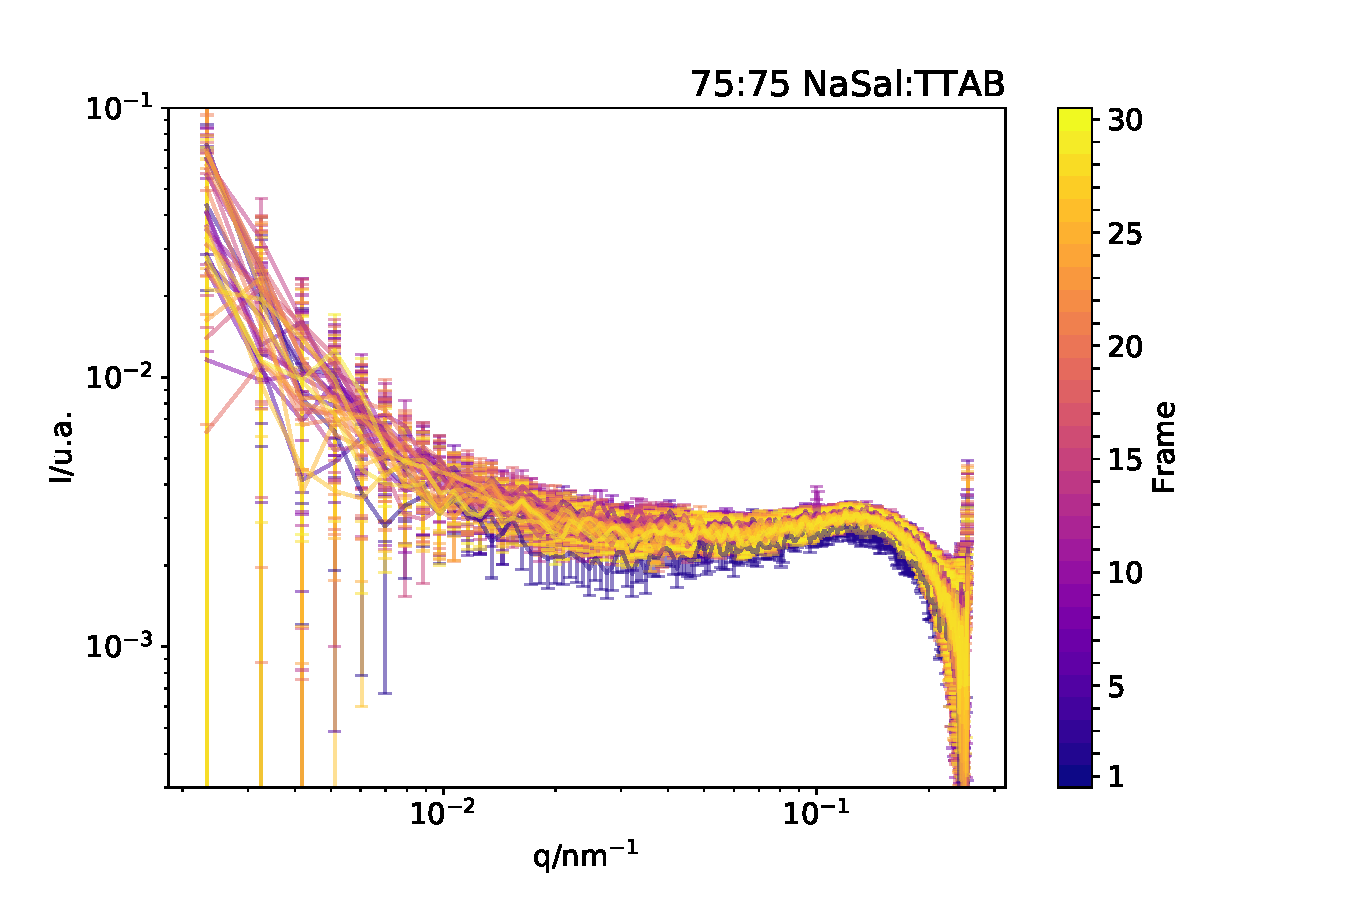
\includegraphics[width=\textwidth]{imagens/saxs/TR_saxs_75_75_dados.pdf}
			\caption{Dados}
			\label{fig:saxs_tr_75_d}
		\end{subfigure}%
		\begin{subfigure}[t]{0.5\textwidth}
			\centering
			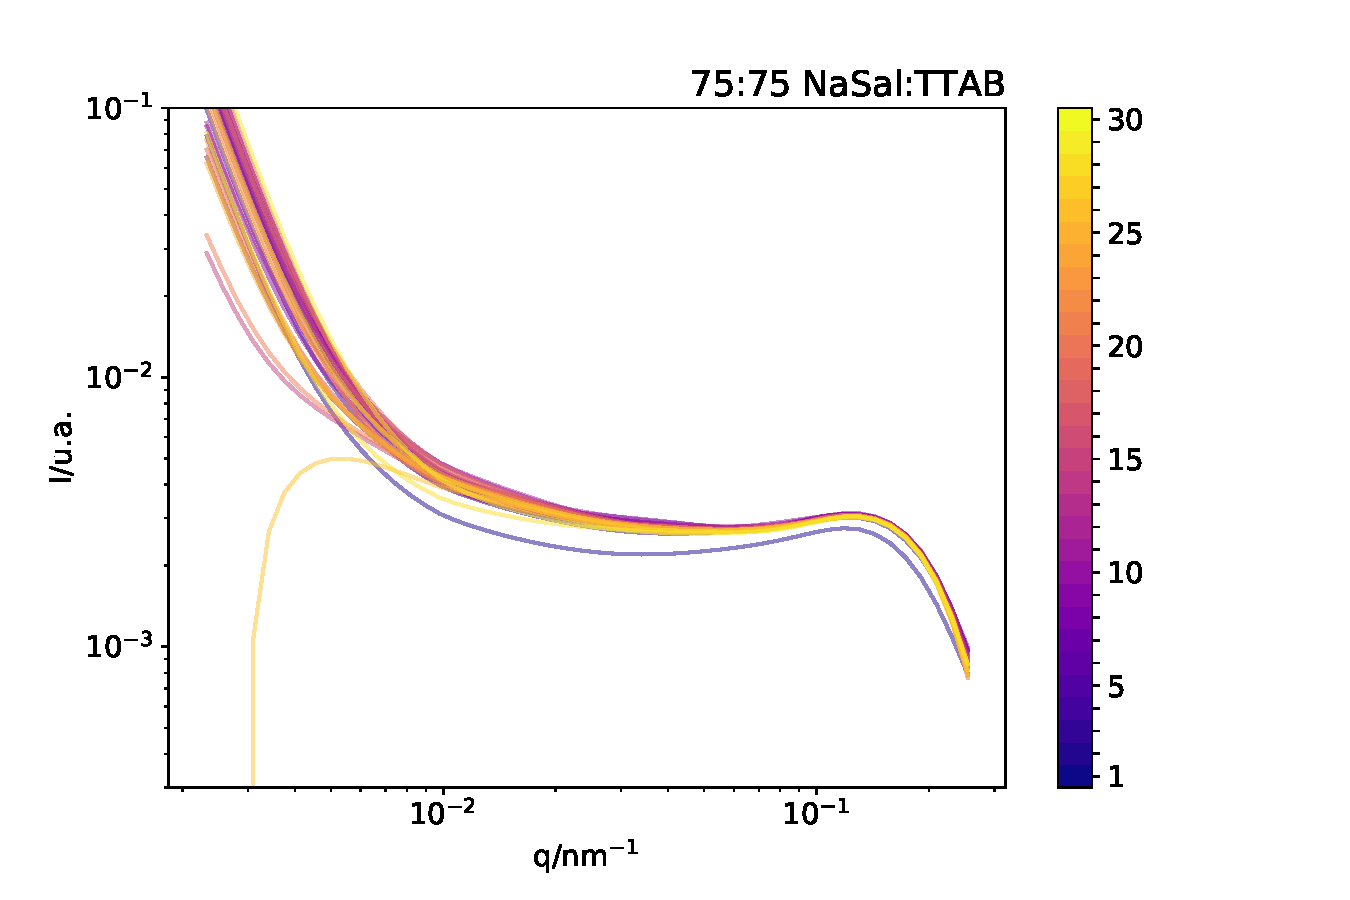
\includegraphics[width=\textwidth]{imagens/saxs/TR_saxs_75_75_ajuste.pdf}
			\caption{Ajustes}
			\label{fig:saxs_tr_a}
		\end{subfigure}
		\caption{Dados experimentais médios das curvas de SAXS nas aquisições numeradas de 1-30, numeradas do menor ao maior tempo de espera. As curvas foram obtidas pela mistura de 75 \mM{} de NaSal com 75 \mM{} de TTAB.}
		\label{fig:saxs_tr_75}
	\end{figure} 
	
	\begin{figure}[h]
		\begin{subfigure}[t]{0.5\textwidth}
			\centering
			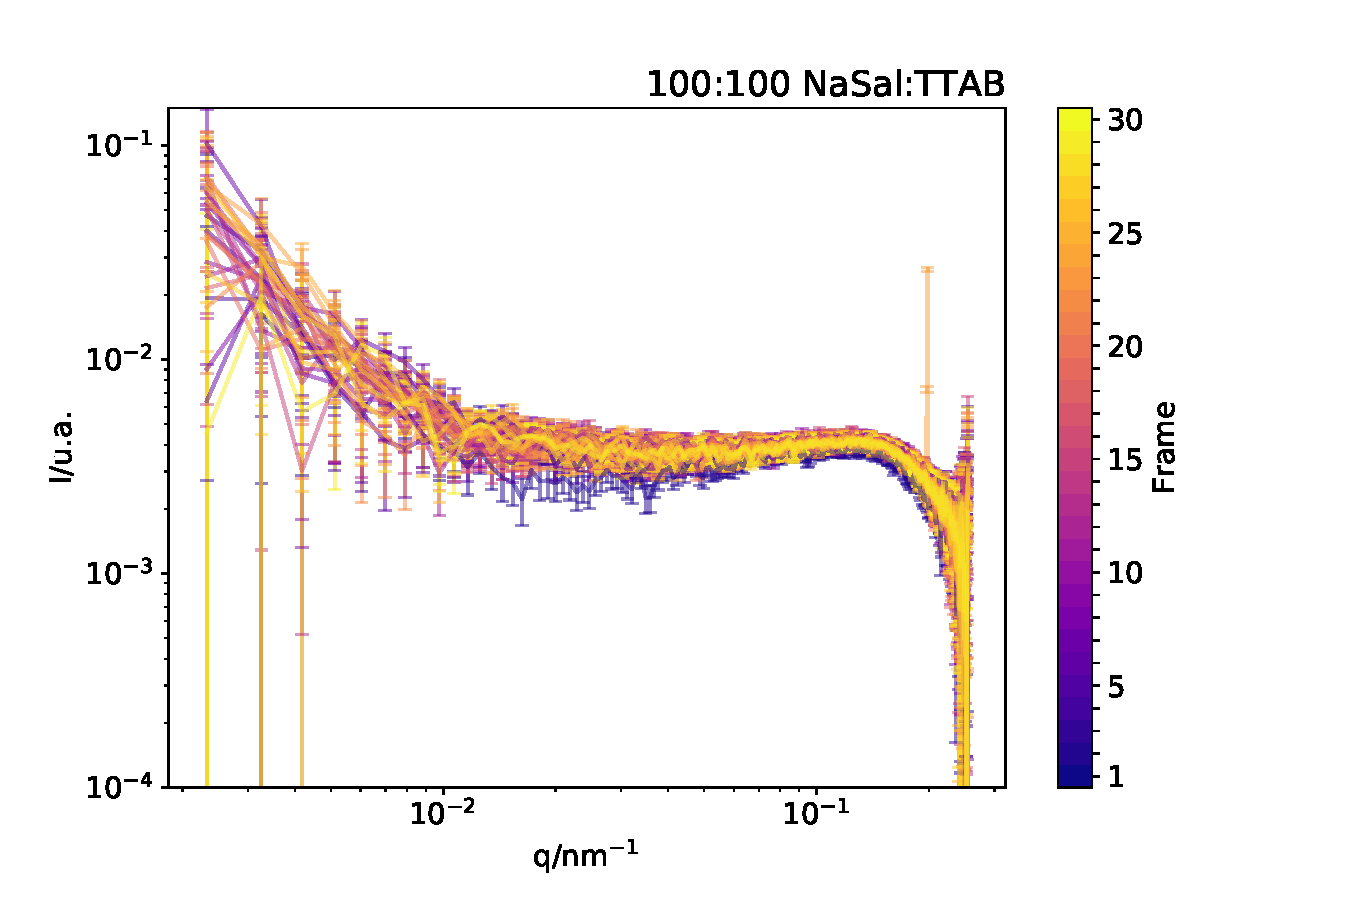
\includegraphics[width=\textwidth]{imagens/saxs/TR_saxs_100_100_dados.pdf}
			\caption{Dados}
			\label{fig:saxs_tr_100_d}
		\end{subfigure}%
		\begin{subfigure}[t]{0.5\textwidth}
			\centering
			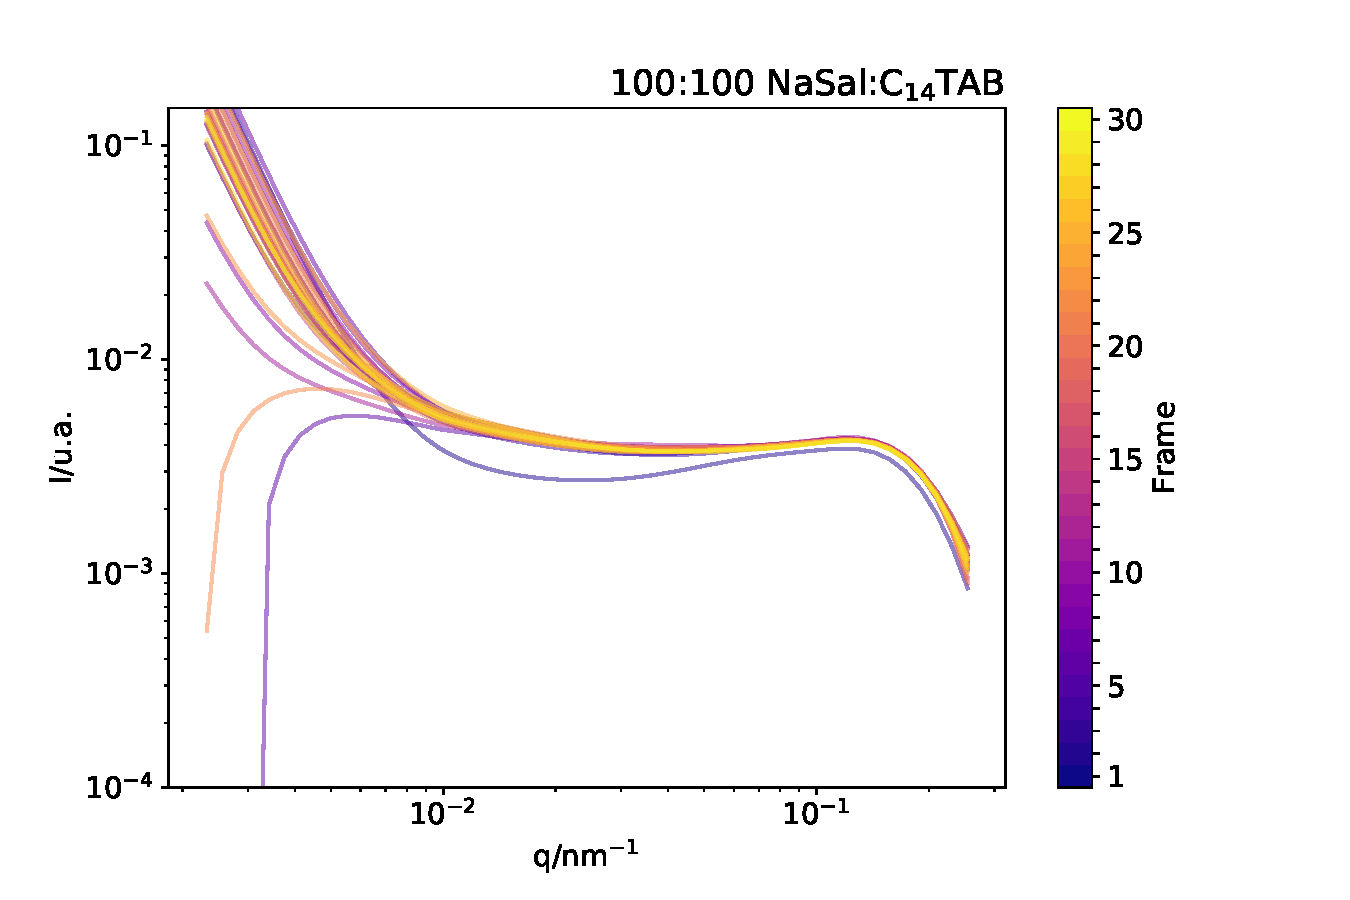
\includegraphics[width=\textwidth]{imagens/saxs/TR_saxs_100_100_ajustes.pdf}
			\caption{Ajustes}
			\label{fig:saxs_tr_100_a}
		\end{subfigure}
		\caption{Dados experimentais médios das curvas de SAXS nas aquisições numeradas de 1-30, numeradas do menor ao maior tempo de espera. As curvas foram obtidas pela mistura de 100 \mM{} de NaSal com 100 \mM{} de TTAB.}
		\label{fig:saxs_tr_100}
	\end{figure} 
	
	\begin{figure}[h]
		\begin{subfigure}[t]{0.5\textwidth}
			\centering
			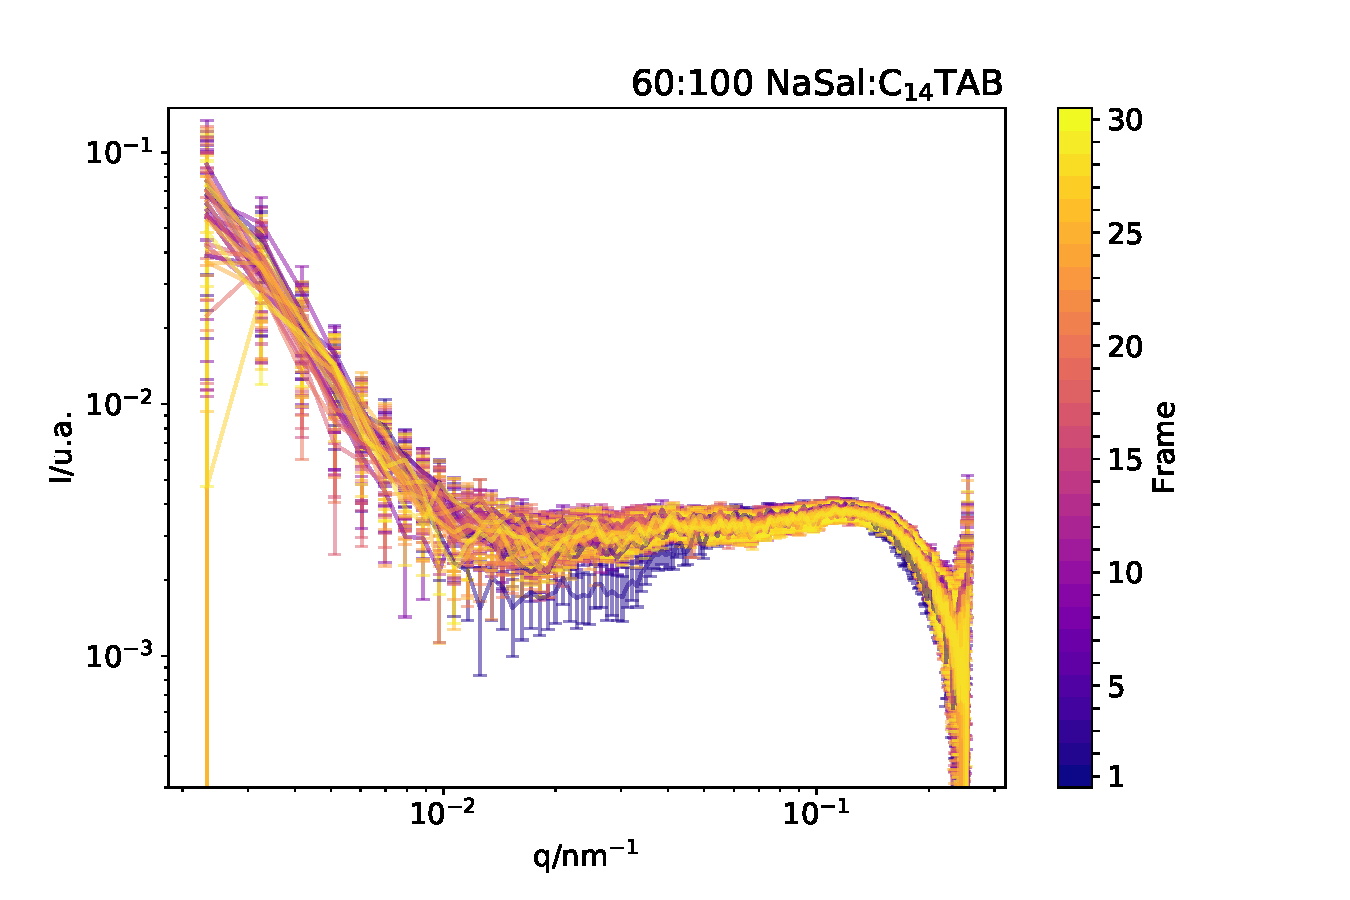
\includegraphics[width=\textwidth]{imagens/saxs/TR_saxs_60_100_3_dados.pdf}
			\caption{Dados}
			\label{fig:saxs_tr_60_3_d}
		\end{subfigure}%
		\begin{subfigure}[t]{0.5\textwidth}
			\centering
			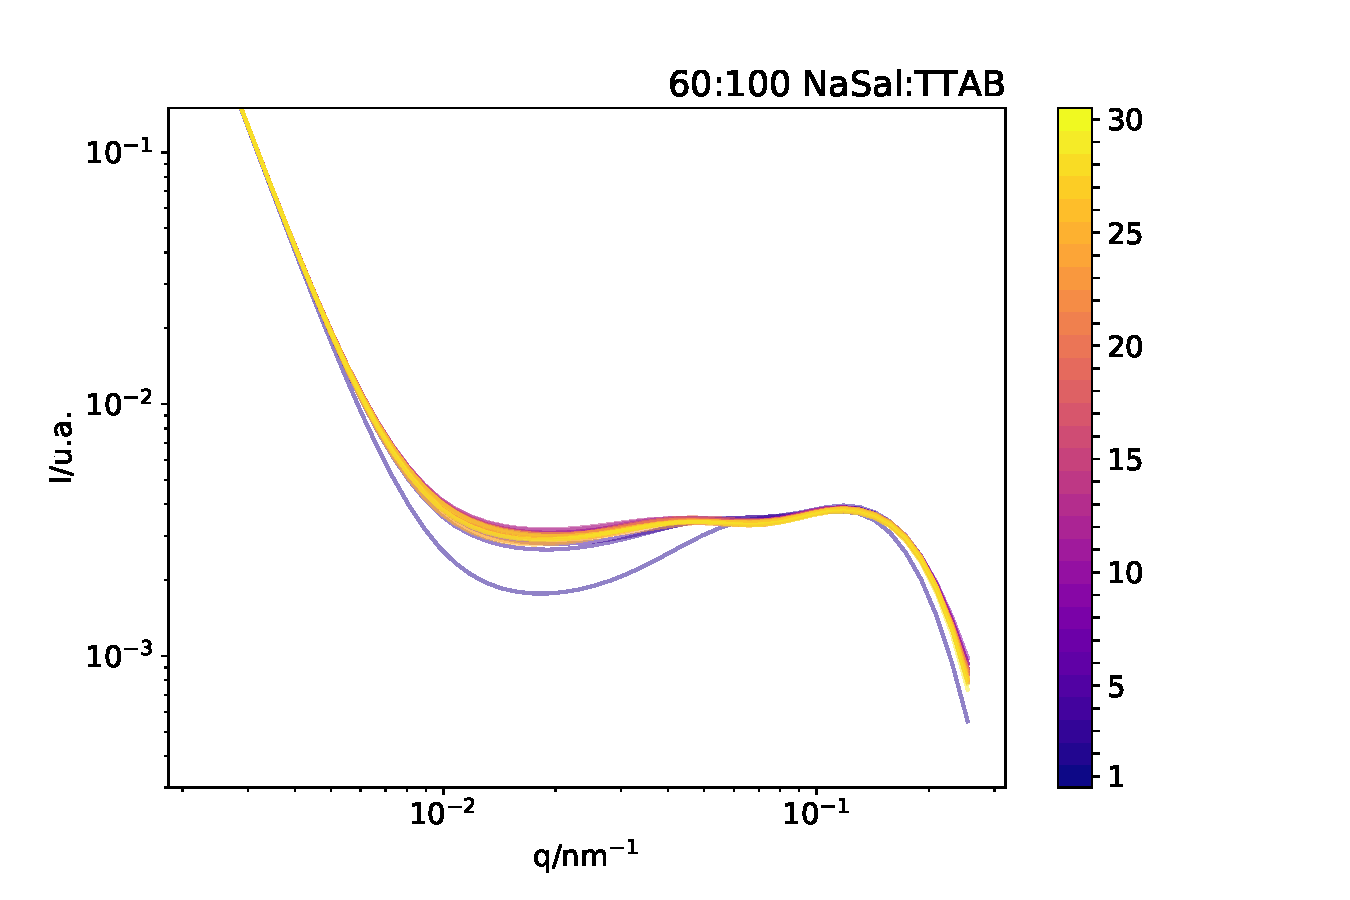
\includegraphics[width=\textwidth]{imagens/saxs/TR_saxs_60_100_3_ajustes.pdf}
			\caption{Ajustes}
			\label{fig:saxs_tr_60_3_a}
		\end{subfigure}
		\caption{Dados experimentais médios das curvas de SAXS nas aquisições numeradas de 1-30, numeradas do menor ao maior tempo de espera. As curvas foram obtidas pela mistura de 60 \mM{} de NaSal com 100 \mM{} de TTAB.}
		\label{fig:saxs_tr_60_3}
	\end{figure} 

	\begin{figure}[h]
		\begin{subfigure}[t]{0.5\textwidth}
			\centering
			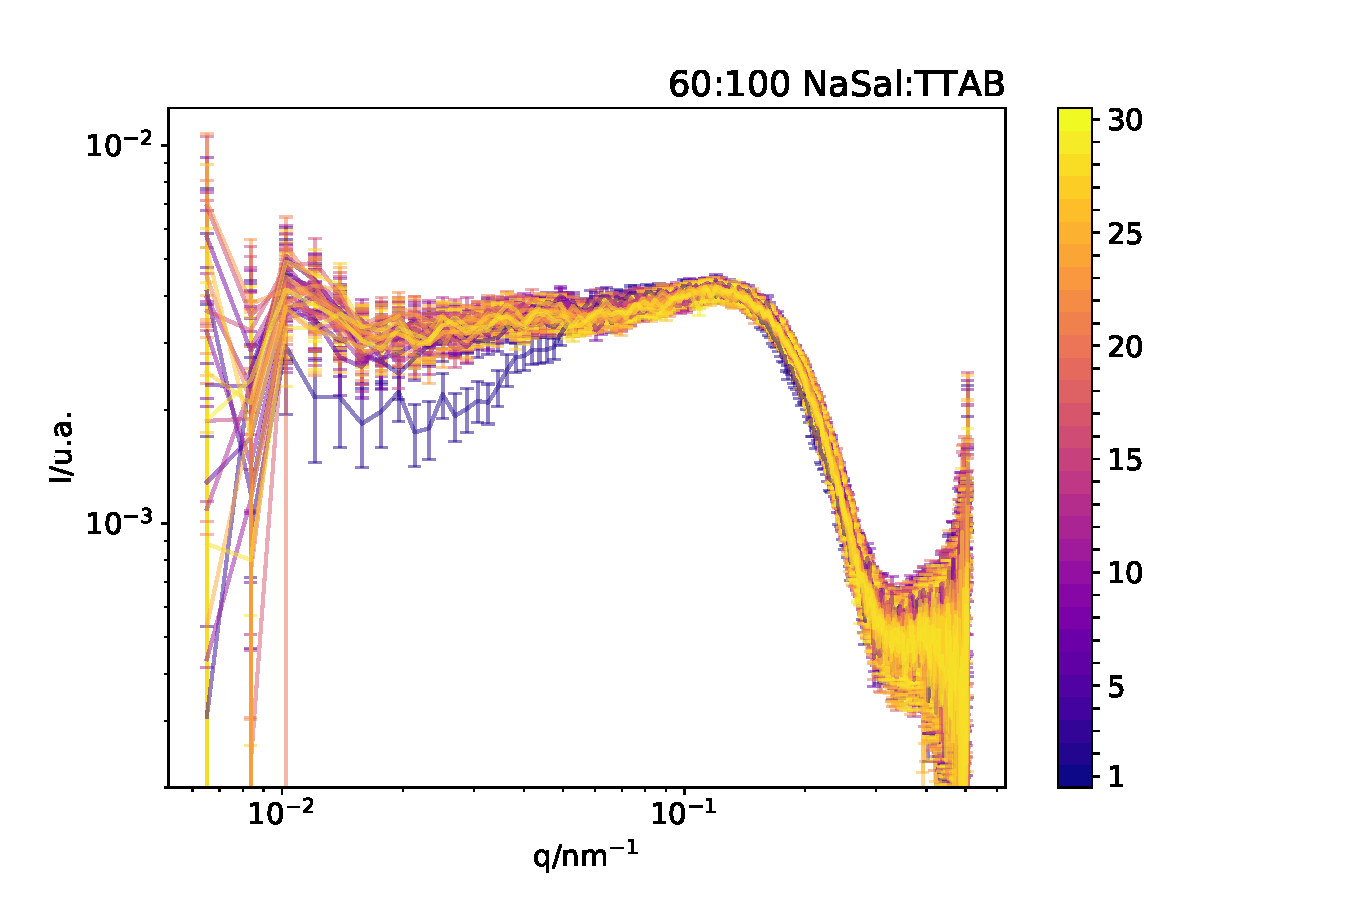
\includegraphics[width=\textwidth]{imagens/saxs/TR_saxs_60_100_15_dados.pdf}
			\caption{Dados}
			\label{fig:saxs_tr_60_15_d}
		\end{subfigure}%
		\begin{subfigure}[t]{0.5\textwidth}
			\centering
			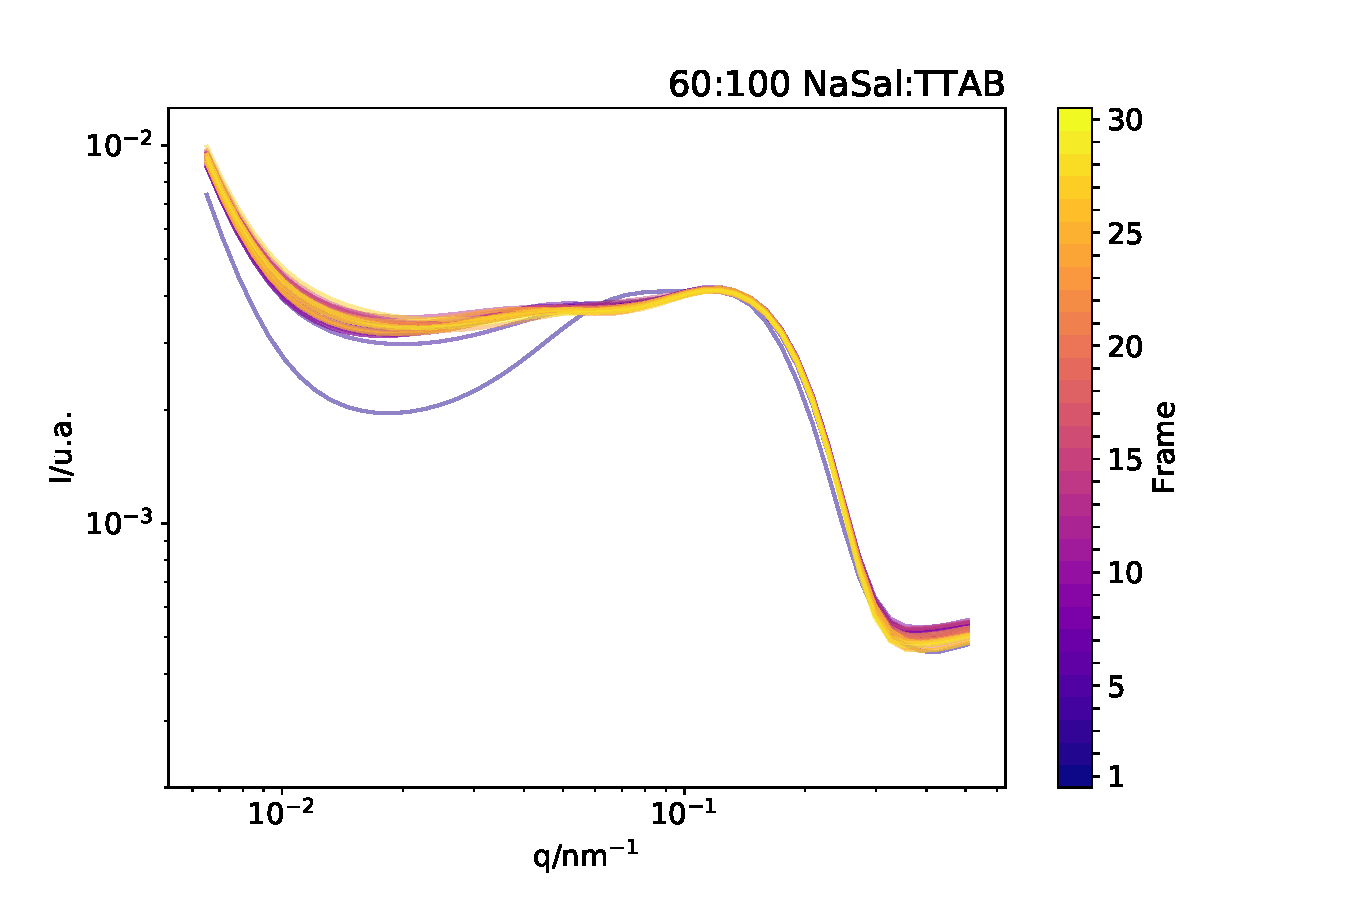
\includegraphics[width=\textwidth]{imagens/saxs/TR_saxs_60_100_15_ajustes.pdf}
			\caption{Ajustes}
			\label{fig:saxs_tr_60_15_a}
		\end{subfigure}
		\caption{Dados experimentais médios das curvas de SAXS nas aquisições numeradas de 1-30, numeradas do menor ao maior tempo de espera. As curvas foram obtidas pela mistura de 60 \mM{} de NaSal com 60 \mM{} de TTAB. Neste caso, a distância do detector é de 1,5m, abrangendo uma faixa de \q{} diferente.}
		\label{fig:saxs_tr_60_15}
	\end{figure} 
	
	Os resultados dos ajustes estão nas figuras 
	
	\begin{figure}
		\centering
		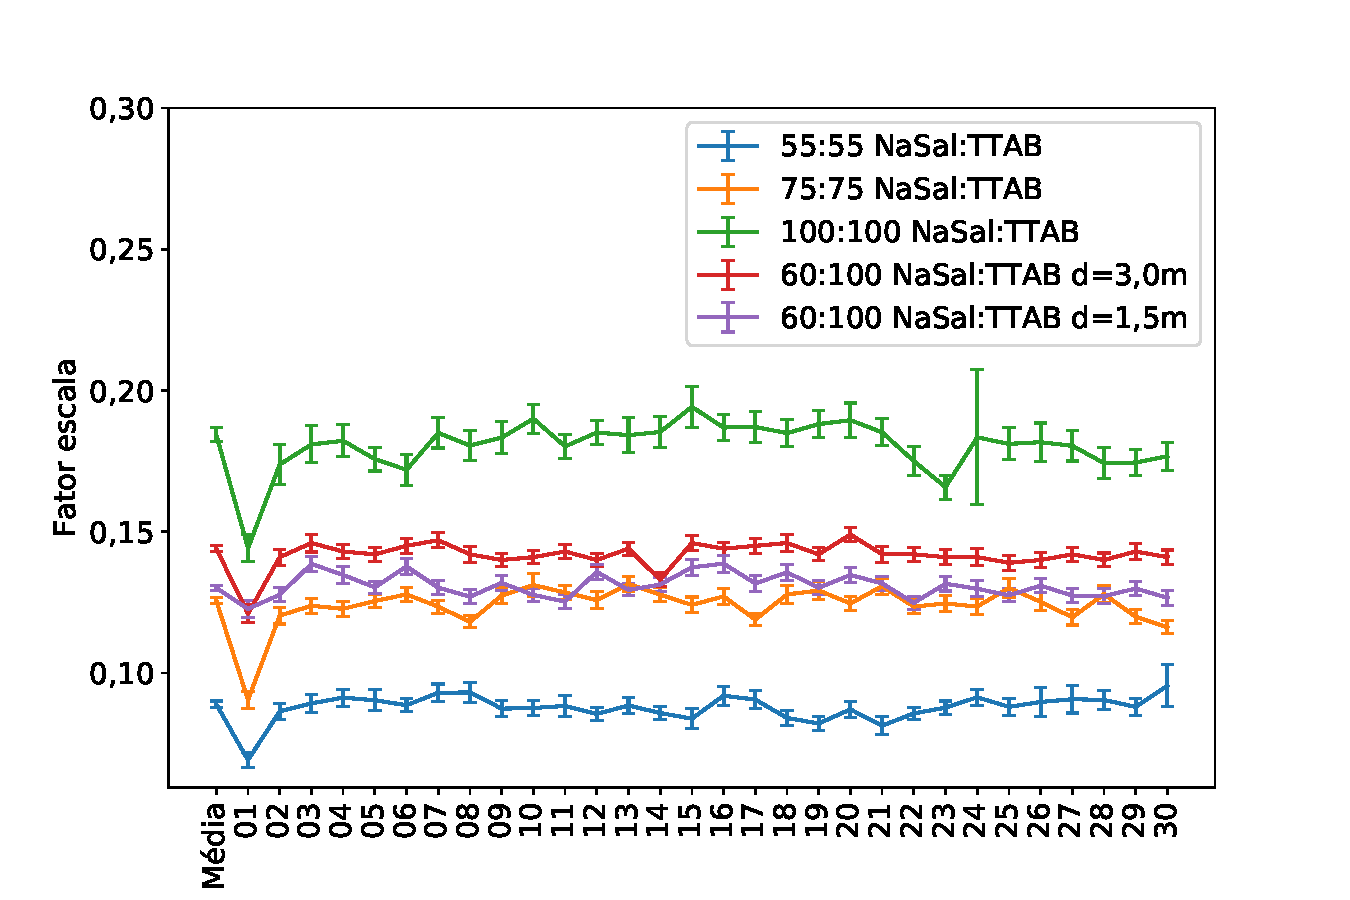
\includegraphics[width=0.7\textwidth]{imagens/saxs/param_scale}
		\caption{}
		\label{fig:param_scale}
	\end{figure}

	\begin{figure}
		\centering
		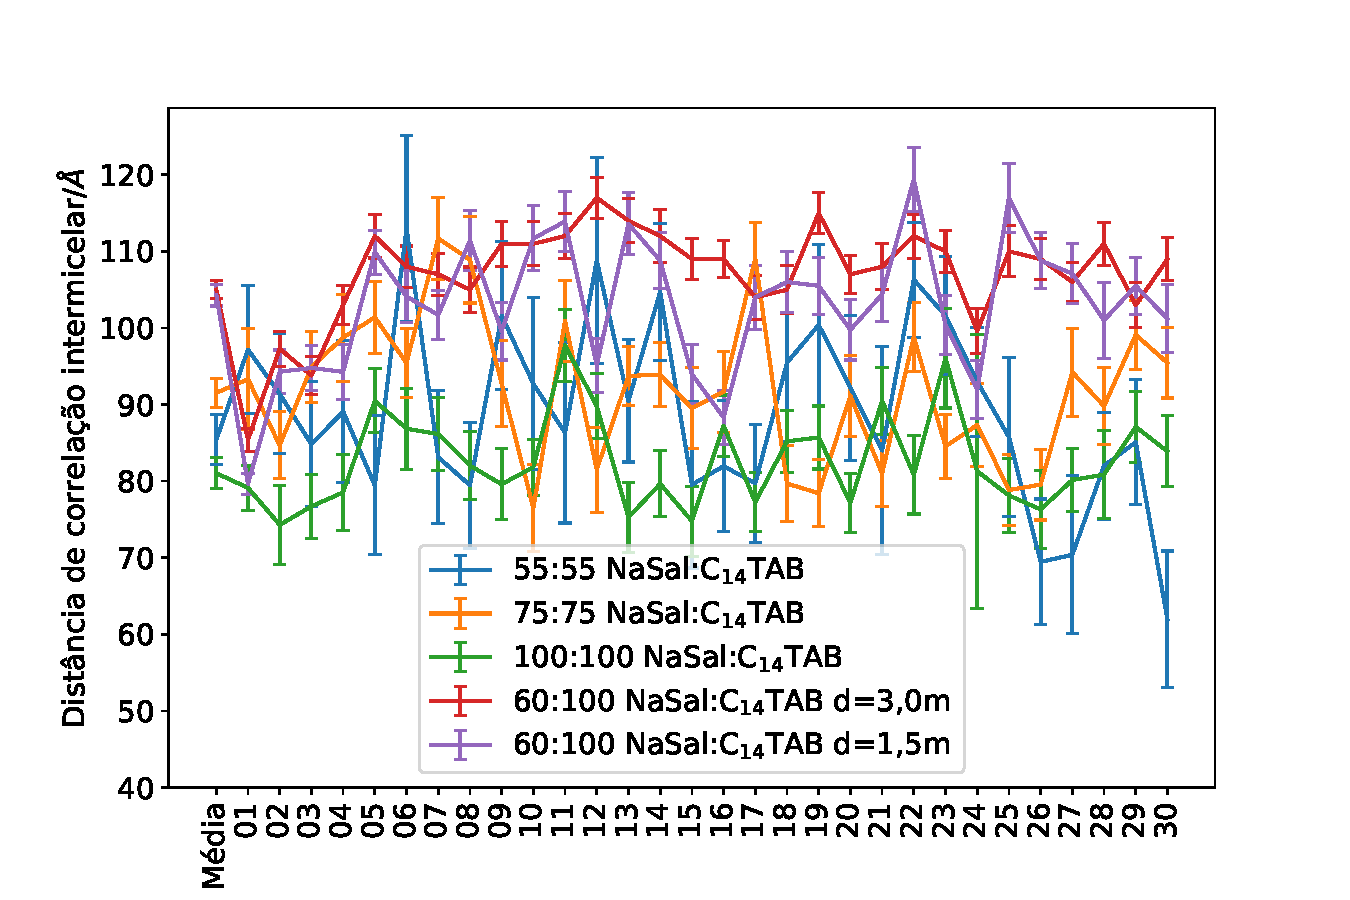
\includegraphics[width=0.7\textwidth]{imagens/saxs/param_d_cq}
		\caption{}
		\label{fig:param_dcq}
	\end{figure}

	\begin{figure}
		\centering
		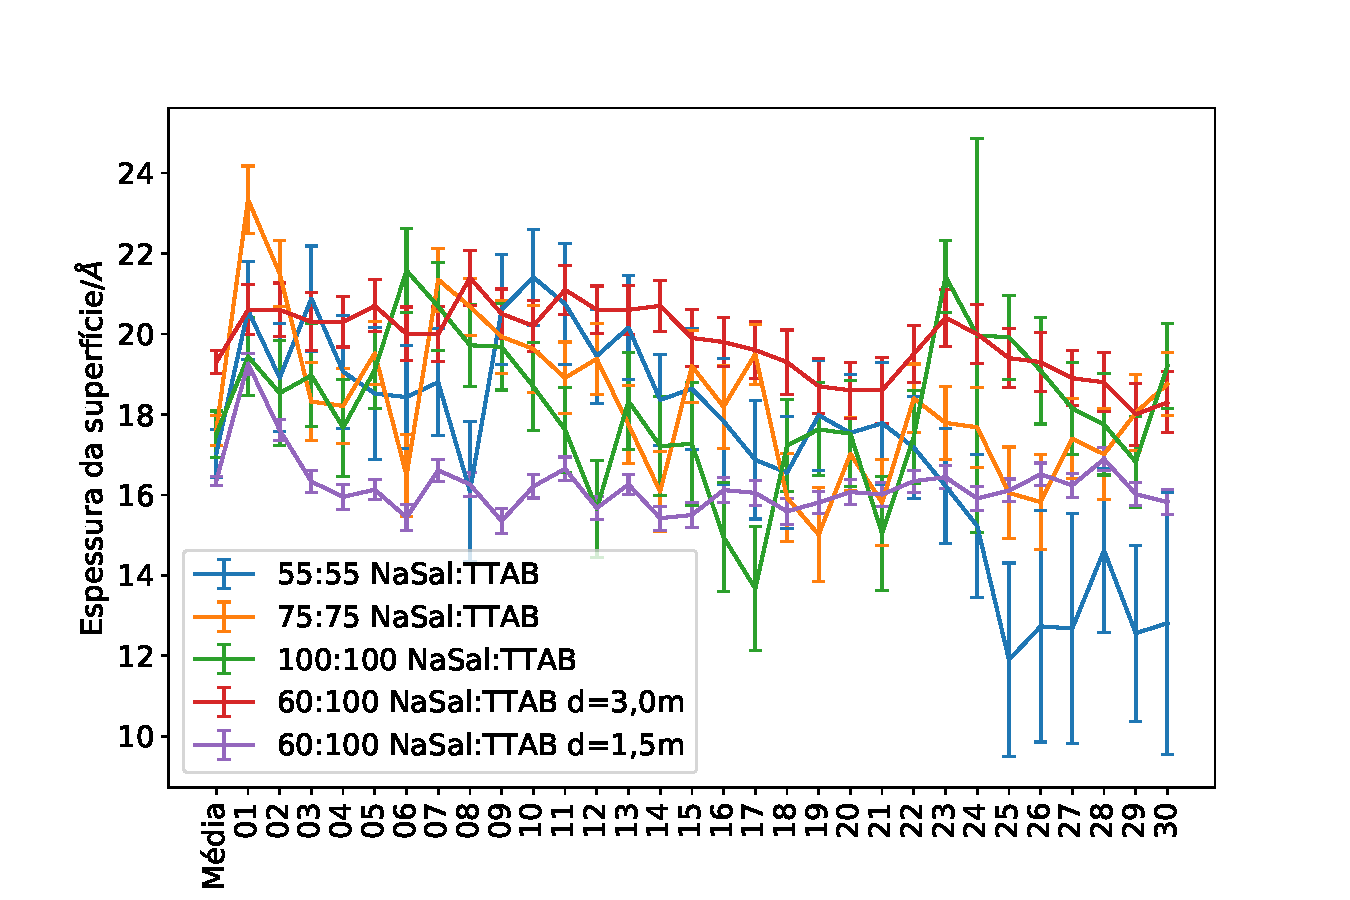
\includegraphics[width=0.7\textwidth]{imagens/saxs/param_d_head}
		\caption{}
		\label{fig:param_dhead}
	\end{figure}

	\begin{figure}
		\centering
		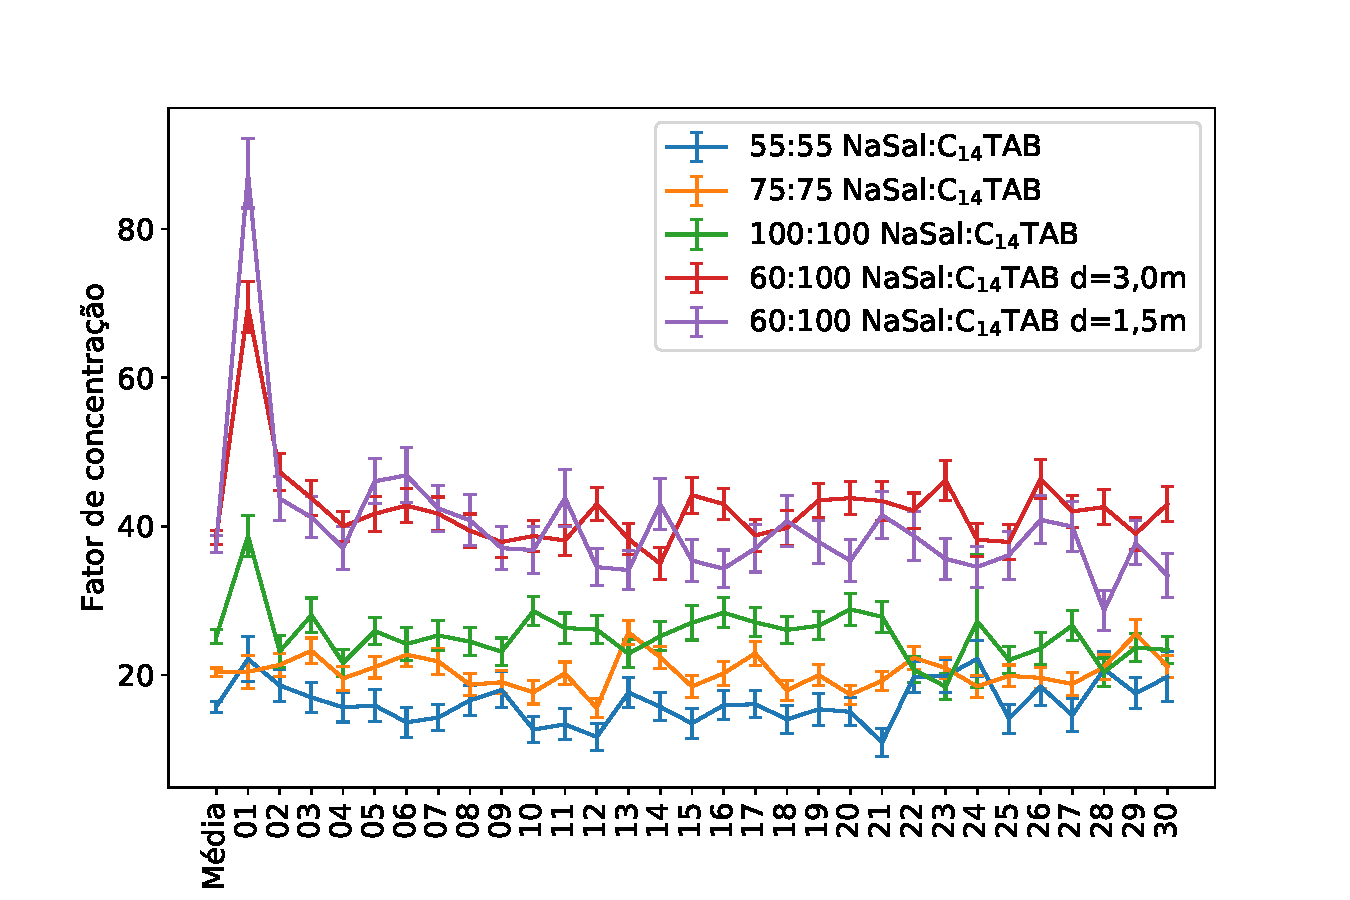
\includegraphics[width=0.7\textwidth]{imagens/saxs/param_nu_rpa}
		\caption{}
		\label{fig:param_nurpa}
	\end{figure}

	\begin{figure}
		\centering
		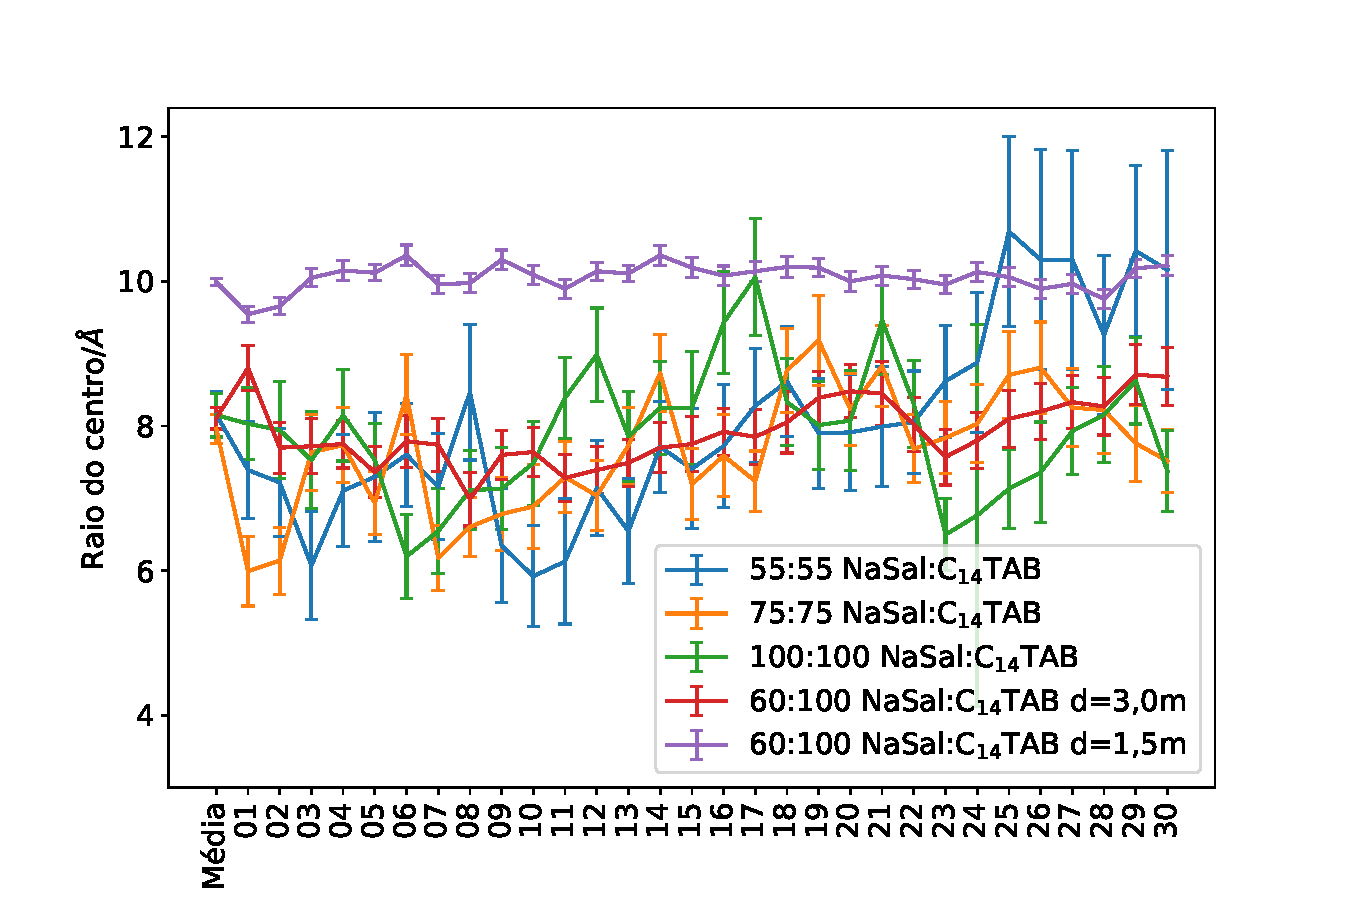
\includegraphics[width=0.7\textwidth]{imagens/saxs/param_rad_core}
		\caption{}
		\label{fig:param_radcore}
	\end{figure}

	\begin{figure}
		\centering
		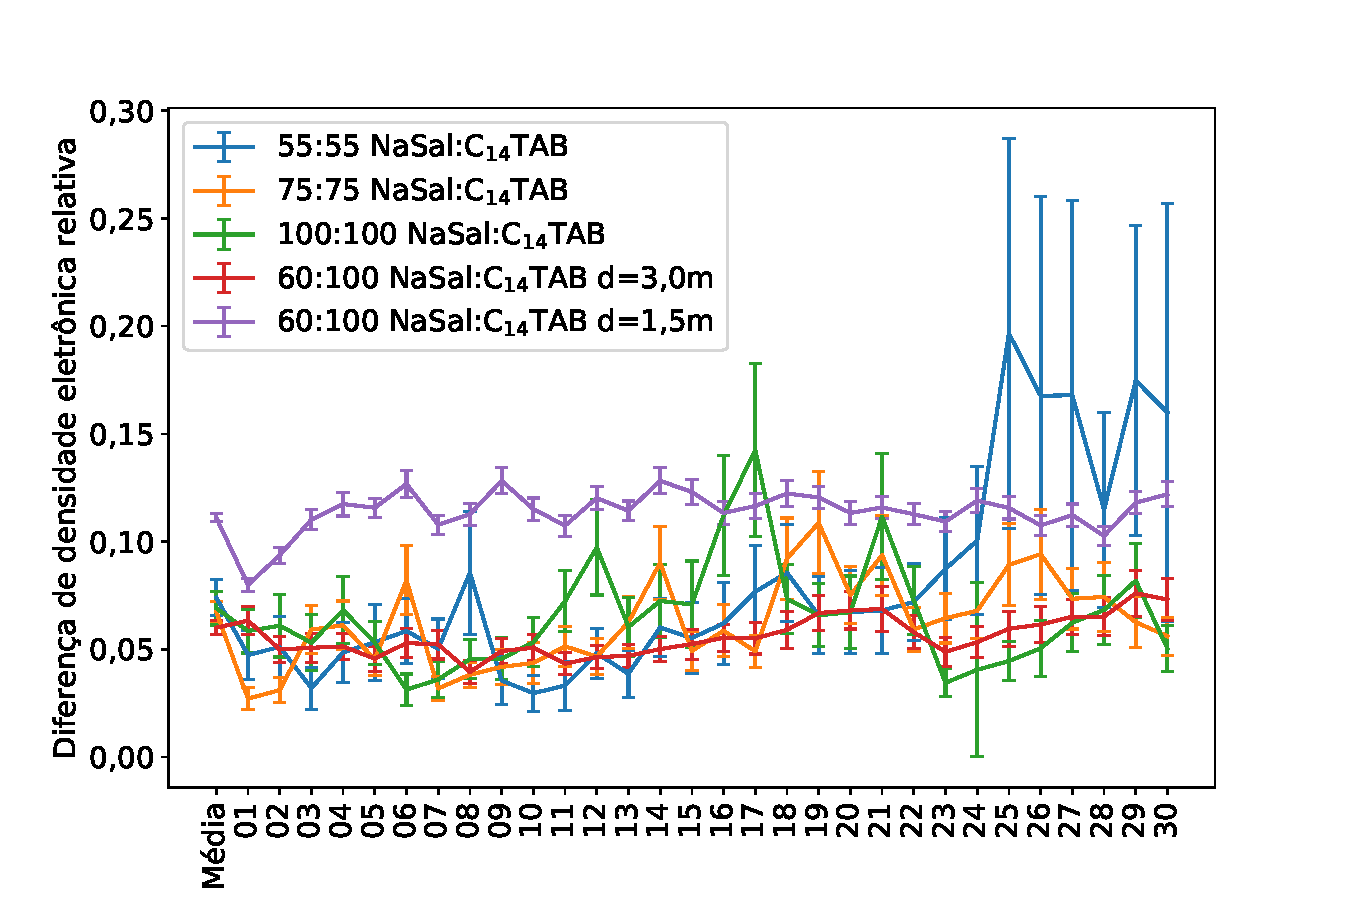
\includegraphics[width=0.7\textwidth]{imagens/saxs/param_rho_rel}
		\caption{}
		\label{fig:param_rhorel}
	\end{figure}
	
			\begin{table}[h]
		\IBGEtab{%
			\caption{Módulos no platô, \(G_0\) em Pa, em função da concentração de NaSal em \mM, de todos os ajustes}
			\label{tab:g0_agua}
		}%
		{%
			\begin{tabular}{c c | c c c c c c}
				\toprule
				            name             & Posição  & Escala                & \(d_{head}\)/nm    & \(r_{core}\)/nm       & \(\rho_{rel}\)        & \(D_{CQ}\)/nm     & \(\nu_{RPA}\)      \\ \midrule
				   \multirow{2}{*}{55:55}    & Média    & 0,089  \(\pm\) 0,001  & 17,0   \(\pm\) 0,6 & 8,2      \(\pm\) 0,3  & 0,074   \(\pm\) 0,008 & 85,0  \(\pm\) 3,0 & 15,8   \(\pm\) 0,7 \\
				                             & Primeiro & 0,069  \(\pm\) 0,003  & 21,0   \(\pm\) 1,0 & 7,4      \(\pm\) 0,7  & 0,05    \(\pm\) 0,01  & 97,0  \(\pm\) 8,0 & 22,0   \(\pm\) 3,0 \\
				   \multirow{2}{*}{75:75}    & Média    & 0,126  \(\pm\) 0,001  & 17,6   \(\pm\) 0,4 & 8,0      \(\pm\) 0,2  & 0,067   \(\pm\) 0,005 & 92,0  \(\pm\) 2,0 & 20,4   \(\pm\) 0,6 \\
				                             & Primeiro & 0,09   \(\pm\) 0,003  & 23,3   \(\pm\) 0,8 & 6,0      \(\pm\) 0,5  & 0,027   \(\pm\) 0,005 & 93,0  \(\pm\) 7,0 & 20,0   \(\pm\) 2,0 \\
				  \multirow{2}{*}{100:100}   & Média    & 0,184  \(\pm\) 0,003  & 17,5   \(\pm\) 0,6 & 8,2      \(\pm\) 0,3  & 0,069   \(\pm\) 0,008 & 81,0  \(\pm\) 2,0 & 25,2   \(\pm\) 0,9 \\
				                             & Primeiro & 0,144  \(\pm\) 0,005  & 19,4   \(\pm\) 1,0 & 8,0      \(\pm\) 0,5  & 0,06    \(\pm\) 0,01  & 79,0  \(\pm\) 3,0 & 39,0   \(\pm\) 3,0 \\
				  \multirow{2}{*}{60:100}    & Média    & 0,144  \(\pm\) 0,001  & 19,3   \(\pm\) 0,3 & 8,1      \(\pm\) 0,2  & 0,06    \(\pm\) 0,003 & 105,0 \(\pm\) 1,0 & 38,5   \(\pm\) 0,9 \\
				                             & Primeiro & 0,121  \(\pm\) 0,003  & 20,6   \(\pm\) 0,6 & 8,8      \(\pm\) 0,3  & 0,063   \(\pm\) 0,006 & 85,0  \(\pm\) 1,0 & 70,0   \(\pm\) 3,0 \\
				\multirow{2}{*}{60:100} 1,5m & Média    & 0,1301 \(\pm\) 0,0009 & 16,4   \(\pm\) 0,1 & 9,99     \(\pm\) 0,05 & 0,111   \(\pm\) 0,002 & 104,0 \(\pm\) 1,0 & 38,0   \(\pm\) 1,0 \\
				                             & Primeiro & 0,123  \(\pm\) 0,003  & 19,3   \(\pm\) 0,3 & 9,5      \(\pm\) 0,1  & 0,08    \(\pm\) 0,003 & 80,0  \(\pm\) 1,0 & 87,0   \(\pm\) 5,0 \\ \bottomrule
			\end{tabular}
		}{}
	\end{table}  
	
	\chapter{Fluorescência resolvida no tempo}